\documentclass[12pt, a4paper, oneside]{ctexart}
\usepackage{amsmath, amsthm, amssymb, bm, color, graphicx, geometry, mathrsfs,extarrows, braket, booktabs, array, xcolor, fontspec, appendix, float, subfigure, wrapfig, enumitem, titlesec}
\usepackage[colorlinks,linkcolor=red,anchorcolor=blue,citecolor=blue,urlcolor=blue,menucolor=black]{hyperref}

%%%% 设置中文字体 %%%%
% fc-list -f "%{family}\n" :lang=zh >d:zhfont.txt 命令查看已有字体
\setCJKmainfont[
    BoldFont=方正黑体_GBK,  % 黑体
    ItalicFont=方正楷体_GBK,  % 楷体
    BoldItalicFont=方正粗楷简体,  % 粗楷体
    Mapping = fullwidth-stop  % 将中文句号“.”全部转化为英文句号“.”,
]{方正书宋简体}  % !!! 注意在Windows中运行请改为“方正书宋简体.ttf” !!!
%%%% 设置英文字体 %%%%
\setmainfont{Minion Pro}
\setsansfont{Calibri}
\setmonofont{Consolas}

%%%% 设置代码块 %%%%
% 在vscode中使用minted需要先配置python解释器, Ctrl+Shift+P, 输入Python: Select Interpreter选择安装了Pygments的Python版本. 再在setting.json中xelatex和pdflatex的参数中加入 "--shell-escape", 即可
% TeXworks中配置方法参考: https://blog.csdn.net/RobertChenGuangzhi/article/details/108140093
\usepackage{minted}
\renewcommand{\theFancyVerbLine}{
    \sffamily\textcolor[rgb]{0.5,0.5,0.5}{\scriptsize\arabic{FancyVerbLine}}} % 修改代码前序号大小
% 加入不同语言的代码块
\newmintinline{cpp}{fontsize=\small, linenos, breaklines, frame=lines}
\newminted{cpp}{fontsize=\small, baselinestretch=1, linenos, breaklines, frame=lines}
\newmintedfile{cpp}{fontsize=\small, baselinestretch=1, linenos, breaklines, frame=lines}
\newmintinline{matlab}{fontsize=\small, linenos, breaklines, frame=lines}
\newminted{matlab}{fontsize=\small, baselinestretch=1, mathescape, linenos, breaklines, frame=lines}
\newmintedfile{matlab}{fontsize=\small, baselinestretch=1, linenos, breaklines, frame=lines}
\newmintinline{python}{fontsize=\small, linenos, breaklines, frame=lines, python3}  % 使用\pythoninline{代码}
\newminted{python}{fontsize=\small, baselinestretch=1, linenos, breaklines, frame=lines, python3}  % 使用\begin{pythoncode}代码\end{pythoncode}
\newmintedfile{python}{fontsize=\small, baselinestretch=1, linenos, breaklines, frame=lines, python3}  % 使用\pythonfile{代码地址}

%%%% 设置行间距与页边距 %%%%
\linespread{1.2}
\geometry{left=2.5cm, right=2.5cm, top=2.5cm, bottom=2.5cm}
% \geometry{left=1.84cm,right=1.84cm,top=2.18cm,bottom=2.18cm}  % 更小的页边距

%%%% 定理类环境的定义 %%%%
\newtheorem{example}{例}            % 整体编号
\newtheorem{theorem}{定理}[section] % 定理按section编号
\newtheorem{definition}{定义}
\newtheorem{axiom}{公理}
\newtheorem{property}{性质}
\newtheorem{proposition}{命题}
\newtheorem{lemma}{引理}
\newtheorem{corollary}{推论}
\newtheorem{condition}{条件}
\newtheorem{conclusion}{结论}
\newtheorem{assumption}{假设}
\numberwithin{equation}{section}  % 公式按section编号 (公式右端的小括号)
\newtheorem{algorithm}{算法}

%%%% 自定义环境 %%%%
\newsavebox{\nameinfo}
\newenvironment{myTitle}[1]{
    \begin{center}
    {\zihao{-2}\bf #1\\}
    \zihao{-4}\it
}{\end{center}}  % \begin{myTitle}{标题内容}作者信息\end{myTitle}
\newcounter{problem}  % 问题序号计数器
\newenvironment{problem}[1][]{\stepcounter{problem}\par\noindent\textbf{题目\arabic{problem}. #1}}{\smallskip\par}
\newenvironment{solution}[1][]{\par\noindent\textbf{#1解答. }}{\smallskip\par}  % 可带一个参数表示题号\begin{solution}{题号}
\newenvironment{note}{\par\noindent\textbf{注记. }}{\smallskip\par}
\newenvironment{remark}{\begin{enumerate}[label=\textbf{注\arabic*.}]}{\end{enumerate}}
\BeforeBeginEnvironment{minted}{\vspace{-0.5cm}}  % 缩小minted环境距上文间距
\AfterEndEnvironment{minted}{\vspace{-0.2cm}}  % 缩小minted环境距下文间距

%%%% 自定义段落开头序号,间距 (titlesec) %%%%
% 中文序号:\zhnum{section}, 阿拉伯序号:\arabic
\titleformat{\section}{\Large\bfseries}{\arabic{section}}{1em}{}[]
\titlespacing{\section}{0pt}{1.2ex plus .0ex minus .0ex}{.6ex plus .0ex}
\titlespacing{\subsection}{0pt}{1.2ex plus .0ex minus .0ex}{.6ex plus .0ex}
\titlespacing{\subsubsection}{0pt}{1.2ex plus .0ex minus .0ex}{.6ex plus .0ex}

%%%% 图片相对路径 %%%%
\graphicspath{{figures/}} % 当前目录下的figures文件夹, {../figures/}则是父目录的figures文件夹
\setlength{\abovecaptionskip}{-0.2cm}  % 缩紧图片标题与图片之间的距离
\setlength{\belowcaptionskip}{0pt} 

%%%% 缩小item,enumerate,description两行间间距 %%%%
\setenumerate[1]{itemsep=0pt,partopsep=0pt,parsep=\parskip,topsep=5pt}
\setitemize[1]{itemsep=0pt,partopsep=0pt,parsep=\parskip,topsep=5pt}
\setdescription{itemsep=0pt,partopsep=0pt,parsep=\parskip,topsep=5pt}

%%%% 自定义公式 %%%%
\everymath{\displaystyle} % 默认全部行间公式, 想要变回行内公式使用\textstyle
\DeclareMathOperator*\uplim{\overline{lim}}     % 定义上极限 \uplim_{}
\DeclareMathOperator*\lowlim{\underline{lim}}   % 定义下极限 \lowlim_{}
\DeclareMathOperator*{\argmax}{arg\,max}  % 定义取最大值的参数 \argmax_{}
\DeclareMathOperator*{\argmin}{arg\,min}  % 定义取最小值的参数 \argmin_{}
\let\leq=\leqslant % 简写小于等于\leq (将全部leq变为leqslant)
\let\geq=\geqslant % 简写大于等于\geq (将全部geq变为geqslant)
\DeclareRobustCommand{\rchi}{{\mathpalette\irchi\relax}}
\newcommand{\irchi}[2]{\raisebox{\depth}{$#1\chi$}} % 使用\rchi将\chi居中

%%%% 一些宏定义 %%%%
\def\bd{\boldsymbol}        % 加粗(向量) boldsymbol
\def\disp{\displaystyle}    % 使用行间公式 displaystyle(默认)
\def\tsty{\textstyle}       % 使用行内公式 textstyle
\def\sign{\text{sign}}      % sign function
\def\wtd{\widetilde}        % 宽波浪线 widetilde
\def\R{\mathbb{R}}          % Real number
\def\N{\mathbb{N}}          % Natural number
\def\Z{\mathbb{Z}}          % Integer number
\def\Q{\mathbb{Q}}          % Rational number
\def\C{\mathbb{C}}          % Complex number
\def\K{\mathbb{K}}          % Number Field
\def\P{\mathbb{P}}          % Polynomial
\def\E{\mathbb{E}}          % Exception
\def\d{\mathrm{d}}          % differential operator
\def\e{\mathrm{e}}          % Euler's number
\def\i{\mathrm{i}}          % imaginary number
\def\re{\mathrm{Re}}        % Real part
\def\im{\mathrm{Im}}        % Imaginary part
\def\res{\mathrm{Res}}      % Residue
\def\ker{\mathrm{Ker}}      % Kernel
\def\vspan{\mathrm{vspan}}  % Span  \span与latex内核代码冲突改为\vspan
\def\L{\mathcal{L}}         % Loss function
\def\O{\mathcal{O}}         % big O notation
\def\wdh{\widehat}          % 宽帽子 widehat
\def\ol{\overline}          % 上横线 overline
\def\ul{\underline}         % 下横线 underline
\def\add{\vspace{1ex}}      % 增加行间距
\def\del{\vspace{-1.5ex}}   % 减少行间距

%%%% 正文开始 %%%%
\begin{document}

%%%% 以下部分是正文 %%%%  
\begin{myTitle}{第二次作业\quad 使用GAN进行CelebA数据集图像填充生成}
    生成式人工智能\\ 吴天阳\ 4124136039\ 人工智能B2480
\end{myTitle}
\section{应用实践}
使用GAN模型在CelebA数据集上进行图像填充实验,并进行改进,以下是各模块代码。
\subsection{模型定义}
基础版的GAN模型生成器采用编码-解码结构,将输入图像通过一系列卷积层降维后再利用转置卷积层还原回原始尺寸,实现图像的生成或重建。判别器则通过多层卷积和全连接层对输入图像进行特征提取与分类,输出图像为真实或生成的概率。代码如下
\begin{pythoncode}
import torch
import torch.nn as nn
from torch.nn.utils import spectral_norm

class Generator(nn.Module):
    def __init__(self):
        super().__init__()

        self.encoder = nn.Sequential(
            nn.Conv2d(3, 64, 4, 2, 1),  # 64x64 -> 32x32
            nn.ReLU(),
            nn.Conv2d(64, 128, 4, 2, 1),  # 32x32 -> 16x16
            nn.BatchNorm2d(128),
            nn.ReLU(),
            nn.Conv2d(128, 256, 4, 2, 1),  # -> 8x8
            nn.BatchNorm2d(256),
            nn.ReLU()
        )

        self.decoder = nn.Sequential(
            nn.ConvTranspose2d(256, 128, 4, 2, 1),  # 8x8 -> 16x16
            nn.BatchNorm2d(128),
            nn.ReLU(),
            nn.ConvTranspose2d(128, 64, 4, 2, 1),   # 16x16 -> 32x32
            nn.BatchNorm2d(64),
            nn.ReLU(),
            nn.ConvTranspose2d(64, 3, 4, 2, 1),     # 32x32 -> 64x64
            nn.Tanh()
        )

    def forward(self, x):
        x = self.encoder(x)
        x = self.decoder(x)
        return x

class Discriminator(nn.Module):
    def __init__(self):
        super().__init__()
        self.main = nn.Sequential(
            nn.Conv2d(3, 64, 4, 2, 1),
            nn.LeakyReLU(0.2),
            nn.Conv2d(64, 128, 4, 2, 1),
            nn.BatchNorm2d(128),
            nn.LeakyReLU(0.2),
            nn.Flatten(),
            nn.Linear(128 * 16 * 16, 1),
            nn.Sigmoid()
        )
    def forward(self, x):
        return self.main(x)

if __name__ == '__main__':
    # Test the models
    G = Generator()
    D = Discriminator()
    
    x = torch.randn(8, 3, 64, 64)  # Batch of 8 images
    fake_images = G(x)
    print("Generator output shape:", fake_images.shape)
    
    D_output = D(fake_images)
    print("Discriminator output shape:", D_output.shape)  # Should be (8, 1) for batch size of 8
\end{pythoncode}

改进版GAN模型在生成器中引入了UNet结构,通过跳跃连接保留了编码器的中间特征,有效提升了生成图像的细节与清晰度。同时,判别器采用PatchGAN架构,并引入谱归一化,增强了训练稳定性和对局部纹理的判别能力,使得模型在保持全局一致性的同时更擅长处理图像局部细节,整体效果优于基础版本。代码如下
\begin{pythoncode}
import torch
import torch.nn as nn
from torch.nn.utils import spectral_norm

# 使用 UNet 结构的生成器,支持 skip-connection,提升细节保留
class UNetGenerator(nn.Module):
    def __init__(self):
        super().__init__()
        # 编码器
        self.enc1 = nn.Sequential(nn.Conv2d(3, 64, 4, 2, 1), nn.ReLU())         # 64x64 -> 32x32
        self.enc2 = nn.Sequential(nn.Conv2d(64, 128, 4, 2, 1), nn.BatchNorm2d(128), nn.ReLU())  # 32->16
        self.enc3 = nn.Sequential(nn.Conv2d(128, 256, 4, 2, 1), nn.BatchNorm2d(256), nn.ReLU()) # 16->8

        # 解码器
        self.dec1 = nn.Sequential(nn.ConvTranspose2d(256, 128, 4, 2, 1), nn.BatchNorm2d(128), nn.ReLU()) # 8->16
        self.dec2 = nn.Sequential(nn.ConvTranspose2d(256, 64, 4, 2, 1), nn.BatchNorm2d(64), nn.ReLU())   # 16->32
        self.dec3 = nn.Sequential(nn.ConvTranspose2d(128, 3, 4, 2, 1), nn.Tanh())                        # 32->64

    def forward(self, x):
        e1 = self.enc1(x)
        e2 = self.enc2(e1)
        e3 = self.enc3(e2)

        d1 = self.dec1(e3)
        d2 = self.dec2(torch.cat([d1, e2], dim=1))
        out = self.dec3(torch.cat([d2, e1], dim=1))
        return out

class PatchDiscriminator(nn.Module):
    def __init__(self):
        super().__init__()
        self.main = nn.Sequential(
            spectral_norm(nn.Conv2d(3, 64, 4, 2, 1)),
            nn.LeakyReLU(0.2),
            spectral_norm(nn.Conv2d(64, 128, 4, 2, 1)),
            nn.LeakyReLU(0.2),
            spectral_norm(nn.Conv2d(128, 256, 4, 2, 1)),
            nn.LeakyReLU(0.2),
            spectral_norm(nn.Conv2d(256, 1, 4, 1, 0)),  # PatchGAN
            nn.Sigmoid()
        )

    def forward(self, x):
        return self.main(x)

# Alias for compatibility
Generator = UNetGenerator
Discriminator = PatchDiscriminator
\end{pythoncode}
\subsection{训练设置}
在训练中,优化模型采用Two Time-Scale Update Rule,将判别器的学习率设为生成器的一半,有助于平衡两者训练速度,避免判别器过快收敛导致生成器训练困难。利用预训练VGG网络提取的高层特征来衡量生成图像与真实图像的感知差异,增强生成图像的结构和语义一致性,提升视觉质量。对生成器使用0.9的平滑标签代替1,提高判别器对真实图像的容错性,从而缓解过拟合并提升稳定性。
\begin{pythoncode}
batch_size = 64
lr = 2e-4
num_epochs = 50
image_size = 64

# 准备数据集
transform = transforms.Compose([
    transforms.CenterCrop(128),
    transforms.Resize(image_size),
    transforms.ToTensor(),
    transforms.Normalize([0.5]*3, [0.5]*3)
])

random_mask_applier = RandomMaskApplier(mask_dir=const.mask_dir, mask_size=(64, 64))
train_dataset = CelebaCustomDataset(
    img_dir=const.celeba_dir,
    transform=transform,
    mask_fn=random_mask_applier.apply_mask,
    train=True
)
eval_dataset = CelebaCustomDataset(
    img_dir=const.celeba_dir,
    transform=transform,
    mask_fn=random_mask_applier.apply_mask,
    train=False
)
train_dataloader = DataLoader(train_dataset, batch_size=batch_size, shuffle=True)
eval_dataloader = DataLoader(eval_dataset, batch_size=batch_size, shuffle=False)

# 模型、损失、优化器
G = Generator().to(device)
D = Discriminator().to(device)
criterion = torch.nn.BCELoss()
l1_loss = torch.nn.L1Loss()
opt_G = torch.optim.Adam(G.parameters(), lr=lr, betas=(0.5, 0.999))  # TTUR G
opt_D = torch.optim.Adam(D.parameters(), lr=lr * 0.5, betas=(0.5, 0.999))  # TTUR D



from torchvision.models import vgg16

# 加载 VGG 感知损失网络
vgg = vgg16(pretrained=True).features[:16].eval().to(device)
for param in vgg.parameters():
    param.requires_grad = False

def perceptual_loss(fake, real):
    return torch.nn.functional.l1_loss(vgg(fake), vgg(real))

from torchvision.models import vgg16

# 感知损失网络
vgg = vgg16(pretrained=True).features[:16].eval().to(device)
for param in vgg.parameters():
    param.requires_grad = False

def perceptual_loss(fake, real):
    return torch.nn.functional.l1_loss(vgg(fake), vgg(real))
\end{pythoncode}
损失函数计算如下:
\begin{pythoncode}
masked, real = masked.to(device), real.to(device)
fake = G(masked)

# 判别器
D_real = D(real).view(-1)
D_fake = D(fake.detach()).view(-1)
loss_D = criterion(D_real, torch.ones_like(D_real)) + \
            criterion(D_fake, torch.zeros_like(D_fake))

opt_D.zero_grad()
loss_D.backward()
opt_D.step()

# 生成器
D_fake = D(fake).view(-1)
vgg_loss = perceptual_loss(fake, real)

# 加上和真实图片的l1损失
loss_G = criterion(D_fake, torch.ones_like(D_fake) * 0.9) + 10 * l1_loss(fake, real) + 0.1 * vgg_loss

opt_G.zero_grad()
loss_G.backward()
opt_G.step()
\end{pythoncode}
\subsection{训练结果}
分别训练两个模型各50个epochs,进行图像填充测试,测试结果如下
\begin{figure}[htbp]
    \centering
    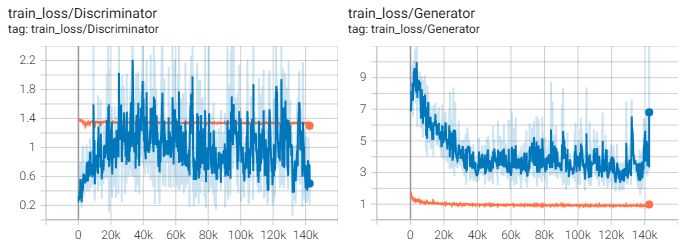
\includegraphics[width=\linewidth]{hw2_train_loss.png}
    \caption{训练集曲线图(蓝色为普通版,橙色为改进版)}
\end{figure}
\begin{figure}[htbp]
    \centering
    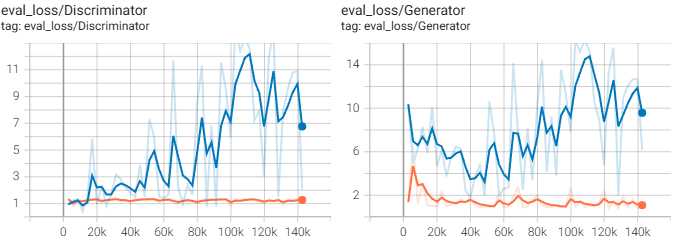
\includegraphics[width=\linewidth]{hw2_eval_loss.png}
    \caption{验证集曲线图(蓝色为普通版,橙色为改进版)}
\end{figure}
\subsection{图像填充效果}
\begin{figure}[H]
  \centering
  \subfigure[普通版生成效果]{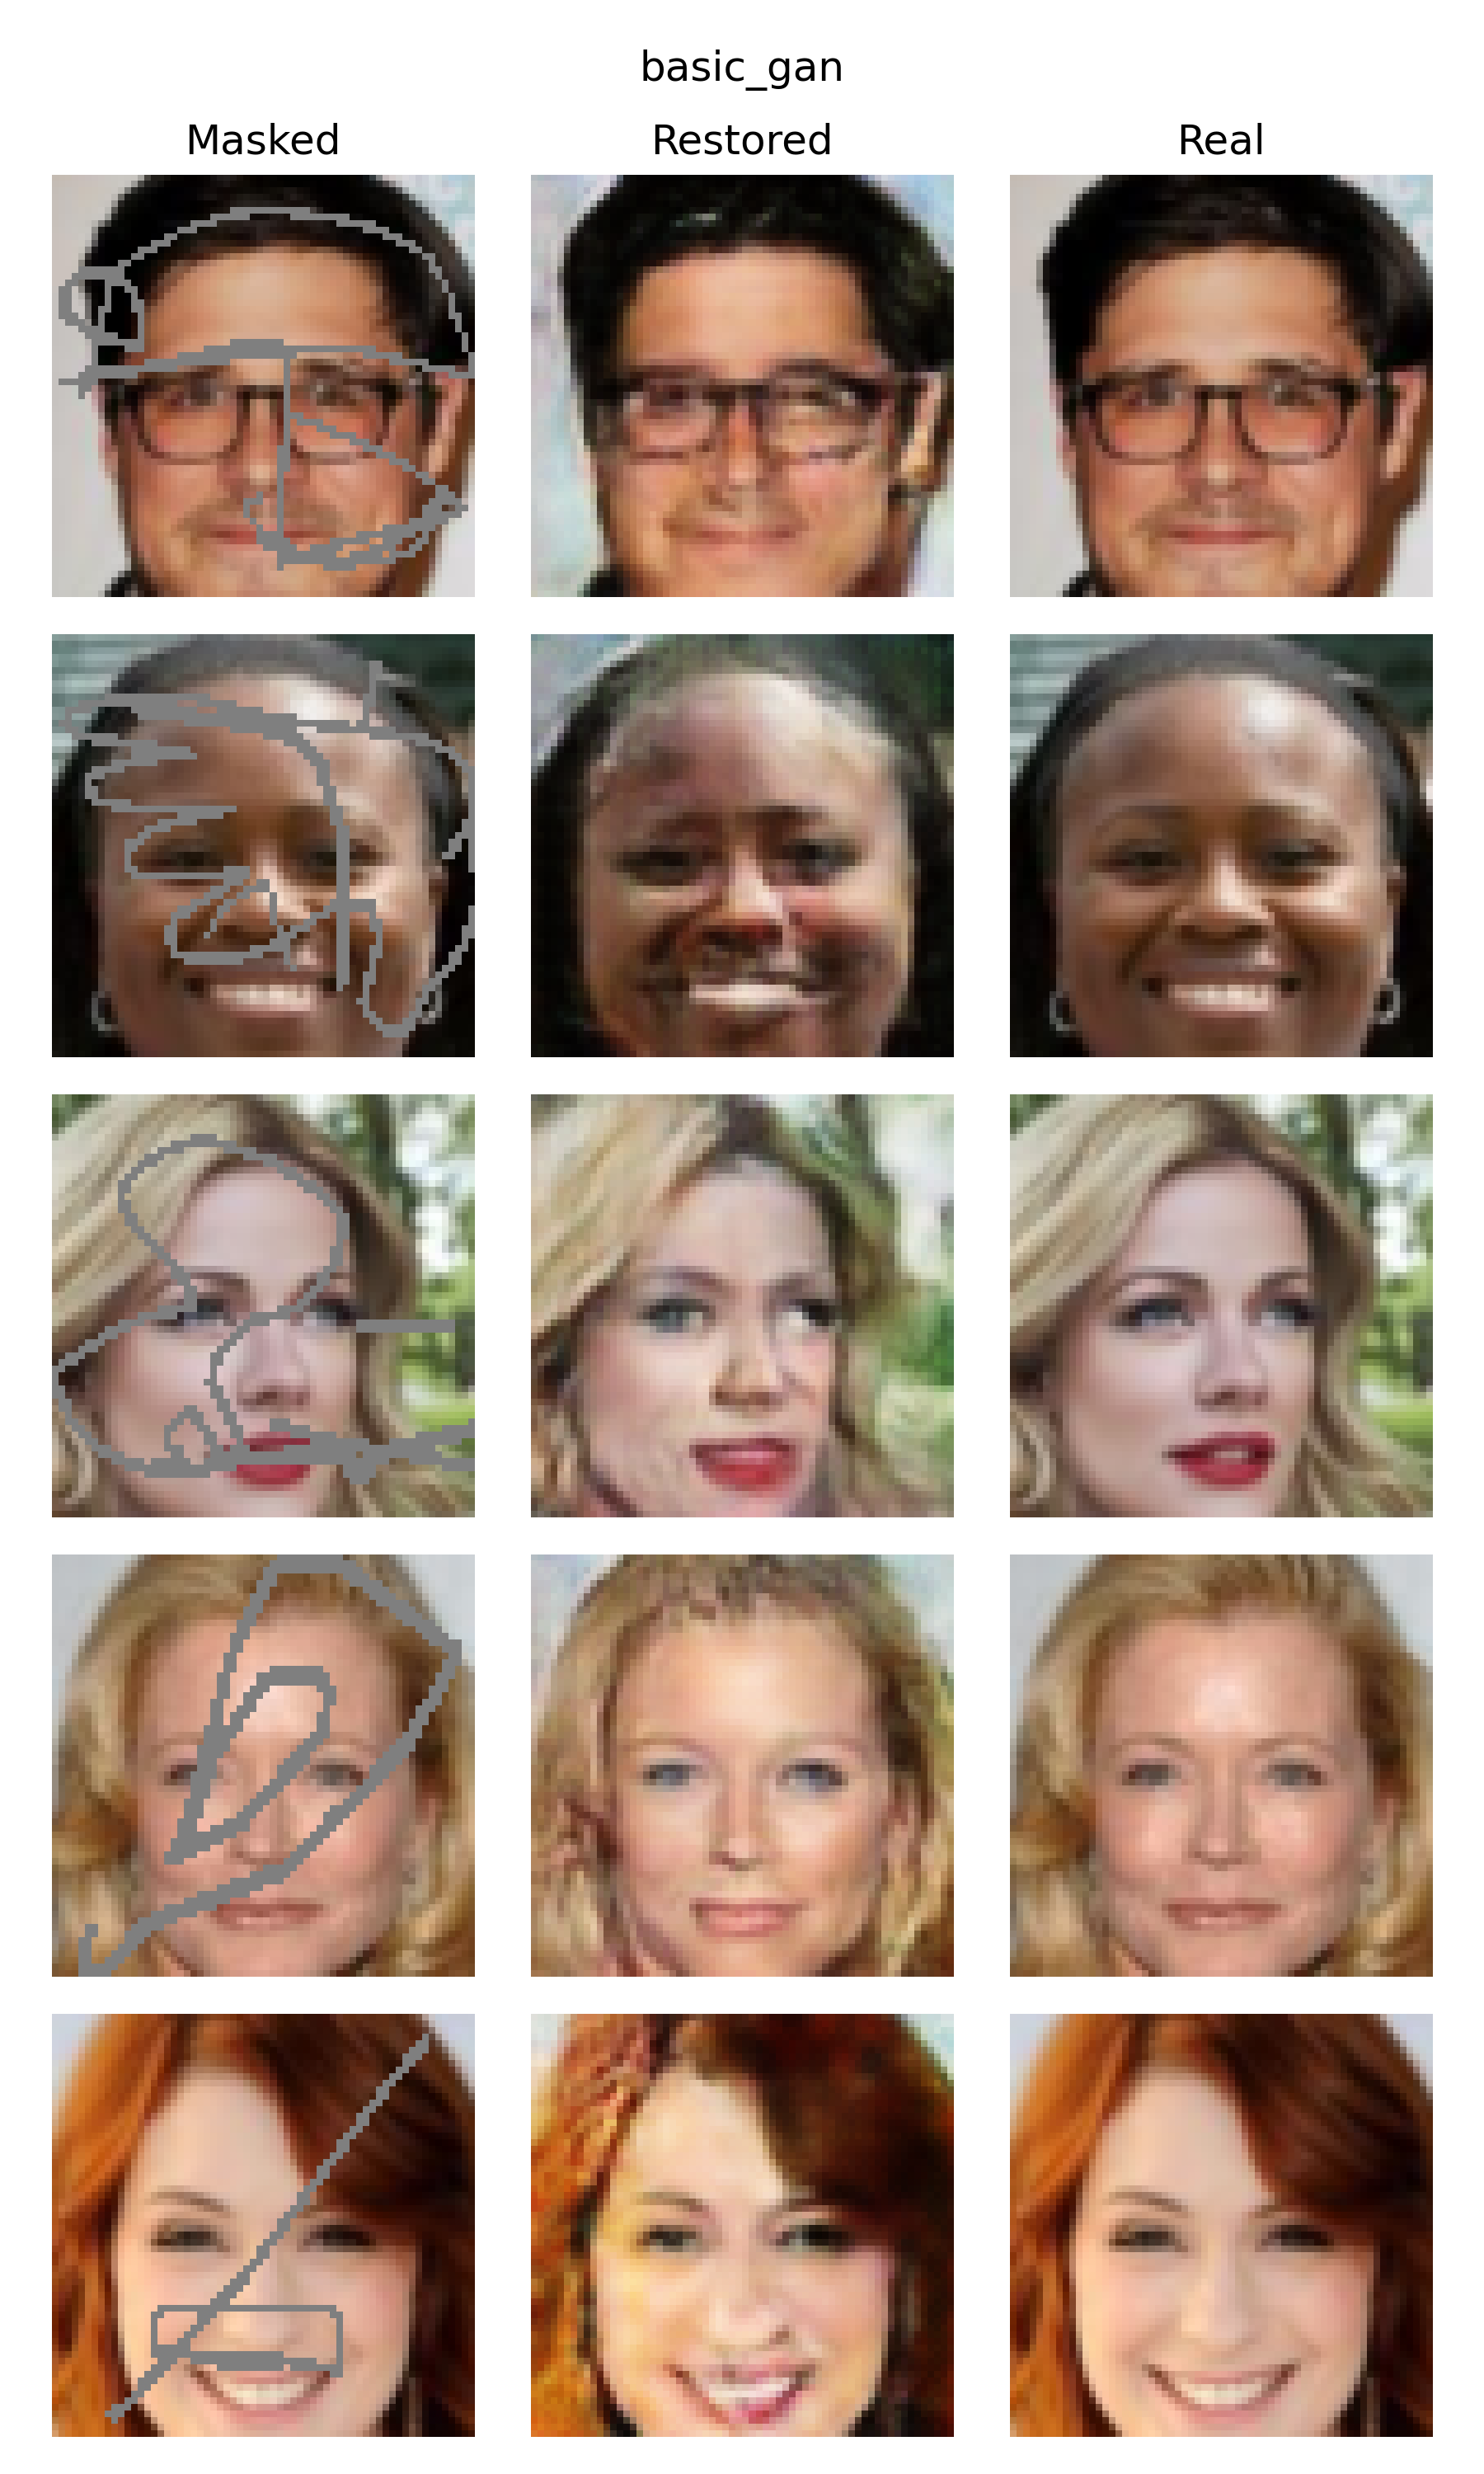
\includegraphics[width=0.49\textwidth]{hw2_eval_basic_gan.png}}
  \subfigure[改进版生成效果]{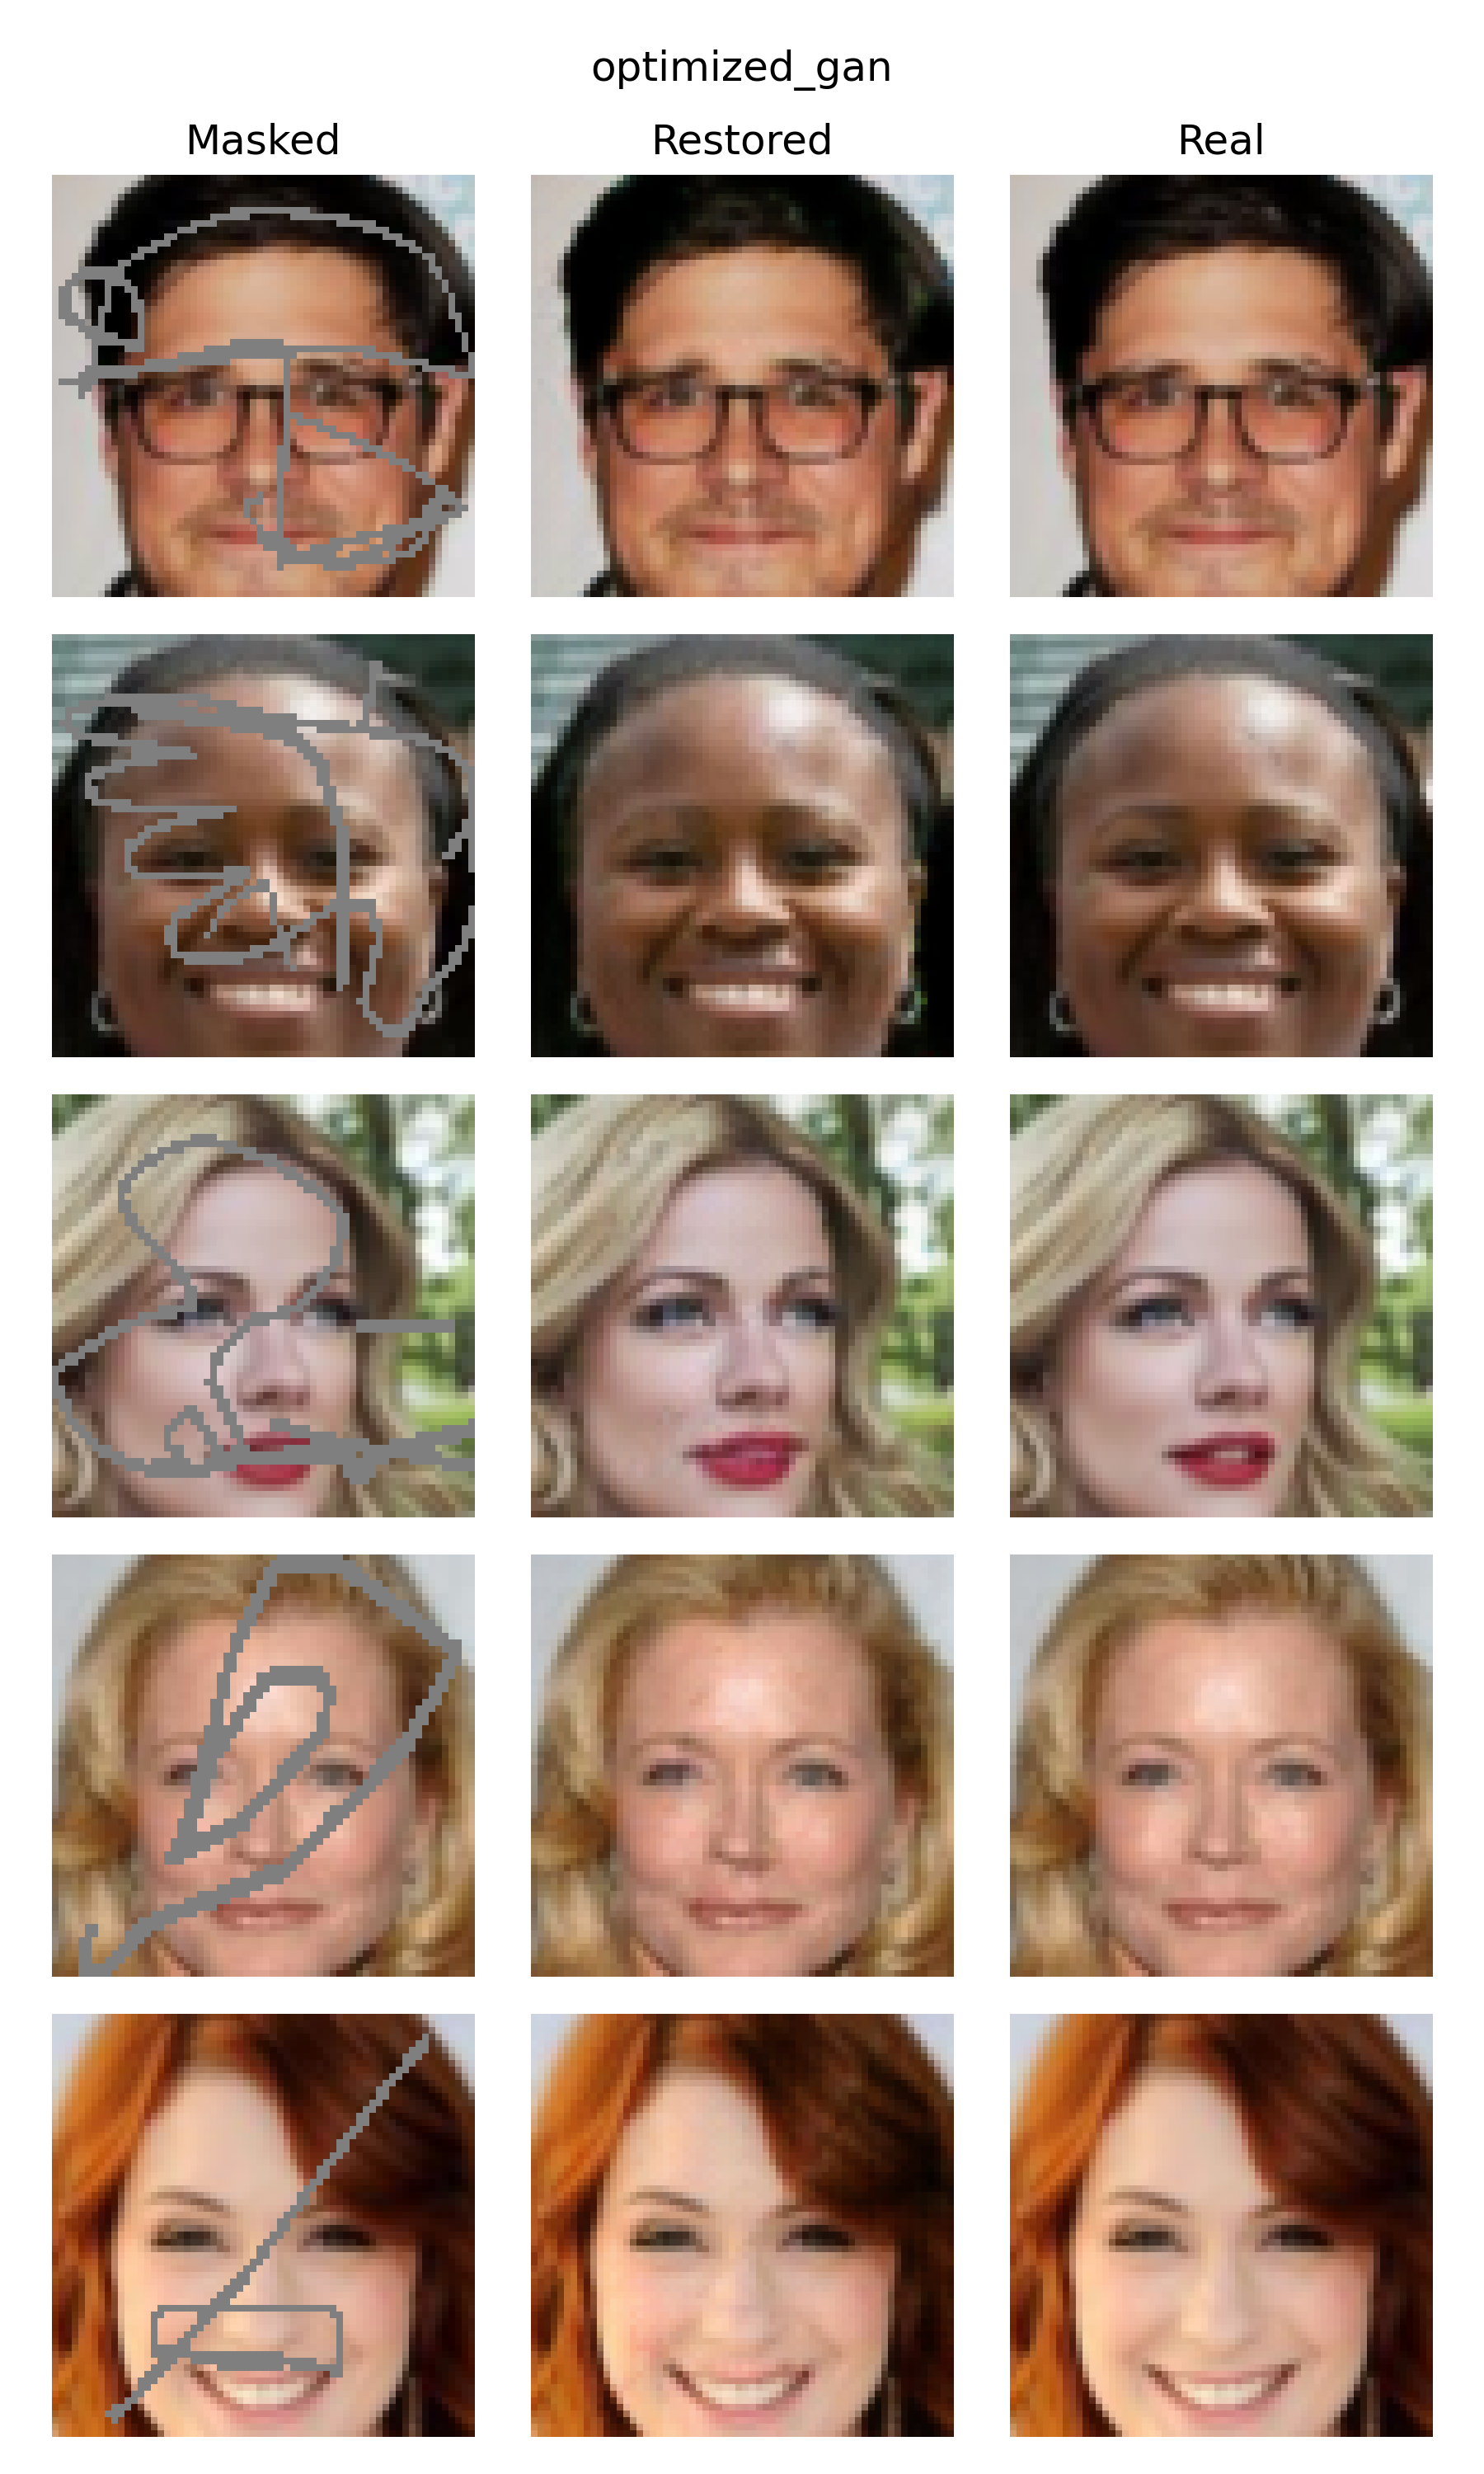
\includegraphics[width=0.49\textwidth]{hw2_eval_optimized_gan.png}}
  \setlength{\abovecaptionskip}{0ex}  % 如果使用了minted会增大图像与标题间距需要进行缩小
  \label{fig-1}
  \caption{图像填充效果对比(左为普通版,右为改进版)}
\end{figure}
可以发现改进版的训练更加稳定,修复后的图像在细节、颜色和结构上更接近真实图像,在遮挡边界的处理更自然,过渡流畅,而基础版会出现模糊、颜色偏差或畸变。
\section{理论分析}
从理论上看,两者的差异主要源于损失函数、优化算法和训练稳定性的改进。基础版模型只使用对抗损失,容易忽略图像的结构与细节,导致还原模糊。优化版本引入感知损失、重建损失等多种辅助项,使模型在保持真实性的同时更好地恢复语义和细节信息。在优化算法上,基础版本采用标准 Adam 优化器,若参数选择不当,训练容易不稳定,而优化版本则引入 RAdam、TTUR 等策略,使生成器与判别器更新更协调。在训练稳定性方面,优化版本结合谱归一化、梯度惩罚等技术,有效缓解模型发散和震荡问题,使最终生成图像更清晰、自然。综合来看,损失设计的合理性、优化器调度机制和稳定性策略的协同是优化后的 GAN 获得更优填充结果的关键。
\end{document}
